\documentclass[12pt,a4paper]{article}

\usepackage[T2A]{fontenc}
\usepackage[utf8]{inputenc}
\usepackage[russian,english]{babel}
\usepackage{indentfirst}
\usepackage{hyperref}
\usepackage{amsmath,amsthm,amstext,amssymb,amscd}
\usepackage{mathtools}
\usepackage{mathrsfs}
\usepackage{graphicx}
\usepackage{caption}
\usepackage{subcaption}

\newcommand*\Laplace{\mathop{}\!\mathbin\bigtriangleup}

\title{Распределение тепла в пластине \\ Метод Якоби}
\author{Игорь Степанов, ФРТК, 213}

\begin{document}

\maketitle
\hrulefill

\section{Постановка задачи}
\label{sec:problem}

Для уравнения 

\begin{equation}
	\Laplace U = -f(x, y), f(x, y) = -2(x^2+y^2) + 2(x+y), U|_{\delta\Omega} = 0
\end{equation}

в области $\Omega = [0,1]\cap[0,1]$ найти распределение тепла в пластине численно. При решении СЛАУ использовать итерационный метод Якоби для равномерной сетки с шагом по обоим направлениям $h \in \{10^{-1}, 10^{-2}, \dots, 10^{-7}\} $ \par

Точное решение имеет вид:

\begin{equation}
	U(x, y) = xy(1-x)(1-y)
\end{equation}

\section{Метод Якоби}
\label{sec:yacobi}

Для метода Якоби используется разностная схема: 
\begin{equation}
	U^{(k+1)}_{i, j} = \frac{1}{4} \left(U^{(k)}_{i - 1, j} + U^{(k)}_{i + 1, j} + U^{(k)}_{i, j - 1} + U^{(k)}_{i, j + 1} - h^2 f_{i, j} \right)
\end{equation}

\section{Результат}
\label{sec:theory}

\begin{tabular}{|l|l|l|l|}

\hline
Шаг h & Точность $\varepsilon$ & Кол-во итераций N & Ошибка err \\
\hline
0.1 & 0.1 & 1 & 0.05771015319824219 \\
0.01 & 0.01 & 1977 & 0.009993698168278047 \\
0.001 & 0.001 & - & - \\
0.0001 & 0.0001 & - & - \\
\hline

\end{tabular}


\begin{figure}
	\centering
	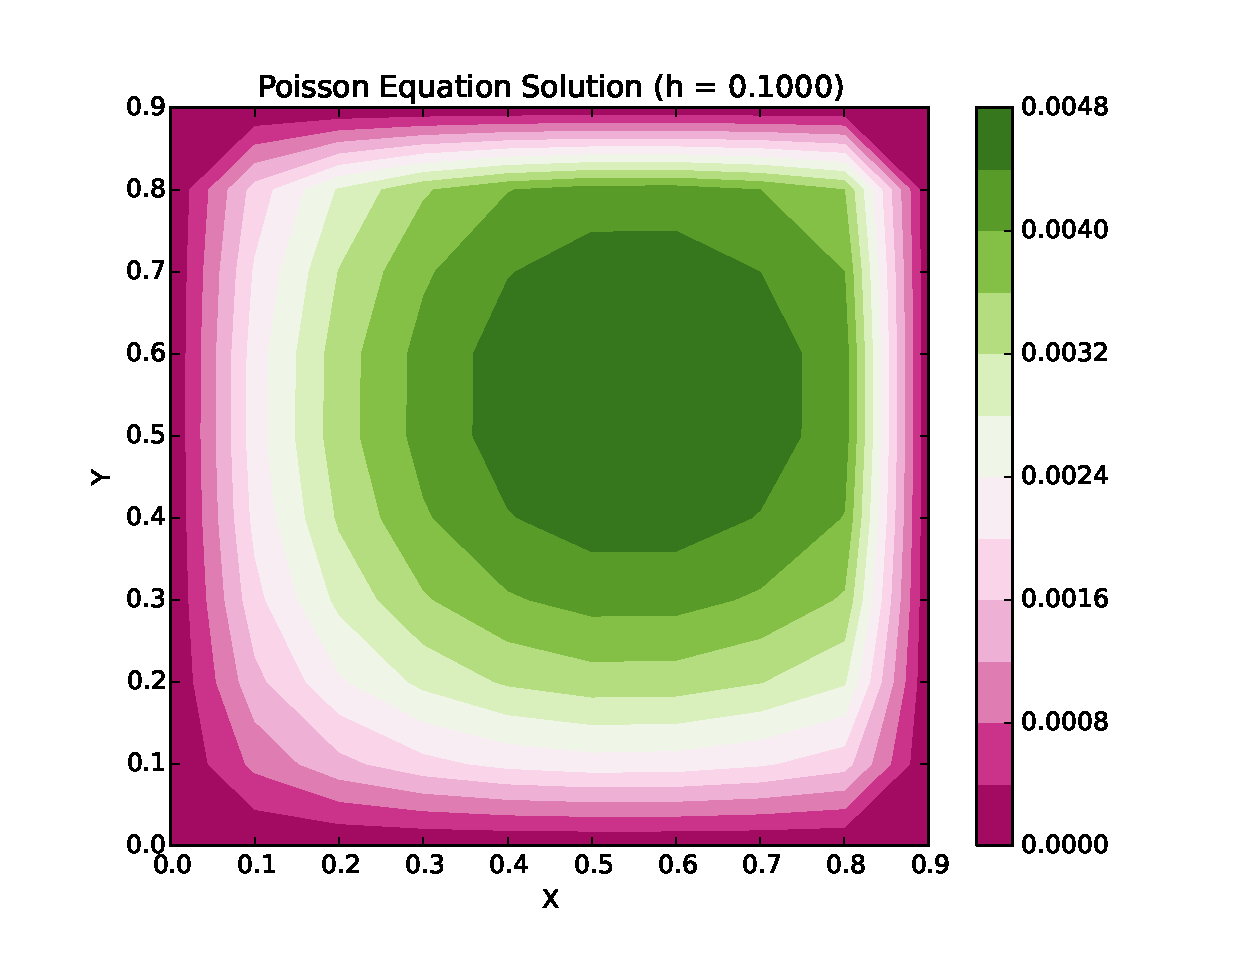
\includegraphics{1_u.eps}
	\caption{Метод Якоби для шага $h=0.1$}\label{fig:u0.1}
\end{figure}

\begin{figure}
	\centering
	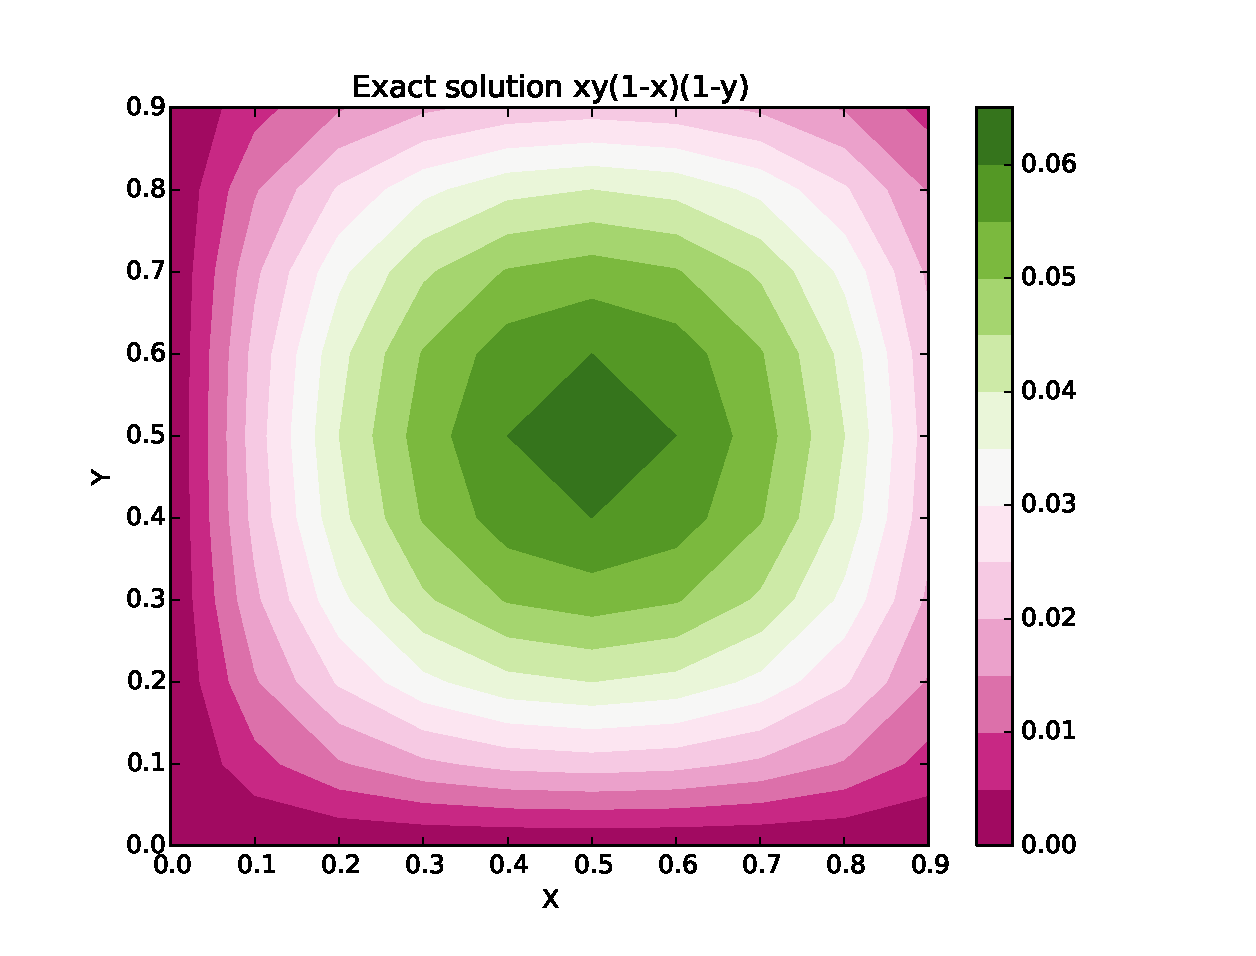
\includegraphics{1_exact.eps}
	\caption{Точное решение}\label{fig:e0.1}
\end{figure}


\section{Заключение}
\label{sec:summary}


% На Рис.~\ref{fig:fig2} показано решение исходной задачи (раздел~\ref{sec:problem}) двухстадийным явным методом Рунге-Кутты (формула \ref{eq:runge-x2}). Сравнивая с Рис.~\ref{fig:fig1}, видно, что решения практически повторяют друг друга, а так как среде Matlab можно доверять, то и наше решение будет верным. \par
% При уменьшении шага примерно до $h \simeq 0.1 $ двухстадийный метод становится непригодным для использования, а Matlab продолжает считать верно. \par

% \begin{figure}
%     \centering
%     \begin{subfigure}[b]{\textwidth}
%         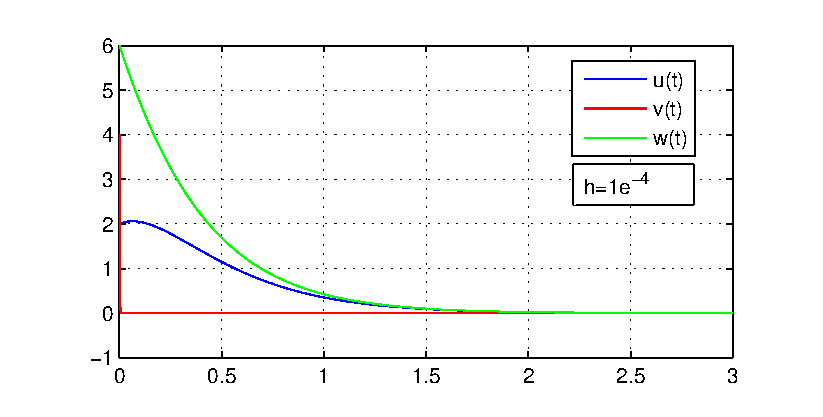
\includegraphics{runge-matlab.eps}
%         \caption{Решение задачи, используя встроенный метод Рунге-Кутты в среде Matlab}
%         \label{fig:fig1}
%     \end{subfigure}
%     \begin{subfigure}[b]{\textwidth}
%         % 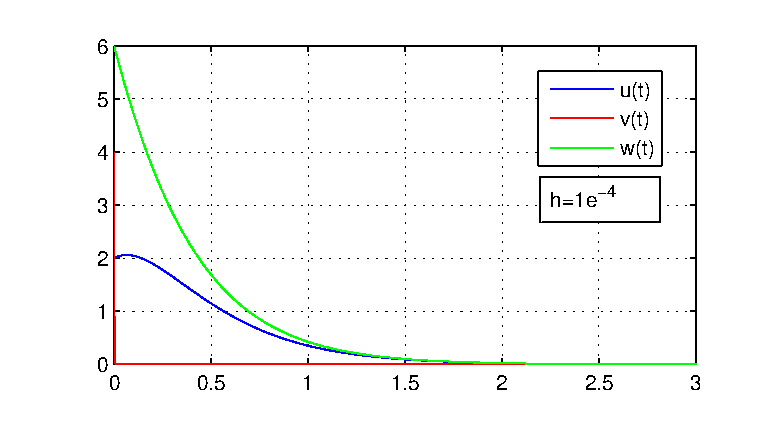
\includegraphics{runge-2x.eps}
%         \caption{Решение задачи, используя двухстадийный явный метод Рунге-Кутты}
%         \label{fig:fig2}
%     \end{subfigure}
%     \caption{Решения задачи}\label{fig:graph}
% \end{figure}

\end{document}
